\documentclass{article}

% if you need to pass options to natbib, use, e.g.:
%     \PassOptionsToPackage{numbers, compress}{natbib}
% before loading neurips_2021

% ready for submission
\usepackage[final]{neurips_2021}

% to compile a preprint version, e.g., for submission to arXiv, add add the
% [preprint] option:
%     \usepackage[preprint]{neurips_2021}

% to compile a camera-ready version, add the [final] option, e.g.:
%     \usepackage[final]{neurips_2021}

% to avoid loading the natbib package, add option nonatbib:
%    \usepackage[nonatbib]{neurips_2021}

\usepackage[utf8]{inputenc} % allow utf-8 input
\usepackage[T1]{fontenc}    % use 8-bit T1 fonts
\usepackage{hyperref}       % hyperlinks
\usepackage{url}            % simple URL typesetting
\usepackage{amsfonts}       % blackboard math symbols
\usepackage{nicefrac}       % compact symbols for 1/2, etc.
\usepackage{xcolor}         % colors
\usepackage{algorithm2e}    % algorithms

% For images
\usepackage{graphicx}
\usepackage{caption}
\usepackage{subcaption}
\usepackage{float}

% Theorem Handling
\usepackage{amsmath,amssymb,amsthm}
\usepackage{cases}
\usepackage{thmtools}
\usepackage{thm-restate}

\declaretheorem{theorem}
\declaretheorem{lemma}
\declaretheorem{proposition}

\newcommand{\R}{\mathbb{R}}
\newcommand{\E}{\mathop{\mathbb{E}}}
\newcommand{\argmin}{\mathop{\text{argmin}}}
\newcommand{\argmax}{\mathop{\text{argmax}}}
\newcommand{\Regret}{\text{Regret}}
\newcommand{\Wealth}{\text{Wealth}}
\newcommand{\diag}{\text{diag}}
\renewcommand{\L}{\mathcal{L}}

\newcommand{\bx}{\mathbf{x}}
\newcommand{\bxt}{\mathbf{\tilde x}}
\newcommand{\by}{\mathbf{y}}
\newcommand{\bw}{\mathbf{w}}
\newcommand{\bz}{\mathbf{z}}
\newcommand{\bv}{\mathbf{v}}
\newcommand{\bg}{\mathbf{g}}
\newcommand{\bu}{\mathbf{u}}
\newcommand{\bq}{\mathbf{q}}
\newcommand{\FTRL}{\text{FTRL}}
\newcommand{\OSD}{\text{OSD}}
\newcommand{\op}{\text{op}}
\renewcommand{\H}{\mathbf{H}}
\newcommand{\todo}[1]{\textcolor{red}{#1}}
\RestyleAlgo{ruled}

\title{A Scale-Free MADGRAD Regret Bound}

% The \author macro works with any number of authors. There are two commands
% used to separate the names and addresses of multiple authors: \And and \AND.
%
% Using \And between authors leaves it to LaTeX to determine where to break the
% lines. Using \AND forces a line break at that point. So, if LaTeX puts 3 of 4
% authors names on the first line, and the last on the second line, try using
% \AND instead of \And before the third author name.

\author{
  Shashank Manjunath \\
  Boston University \\
  \texttt{manjuns@bu.edu} \\
}

\begin{document}

\maketitle

\begin{abstract}
  We introduce a new convergence bound for the MADGRAD optimization algorithm which requires no assumption of the
  boundedness of gradients. MADGRAD, an optimization algorithm in the family of AdaGrad adaptive gradient methods, shows
  promising results on deep learning optimization problems, outperforming Adam and providing a provable convergence
  bound (\cite{defazio_adaptivity_nodate}). We additionally show emprical results of MADGRAD and Modernized Dual
  Averaging (MDA) (\cite{jelassi_dual_2020}) in comparison to Adam and SGD on the CIFAR10
  dataset (\cite{krizhevsky_learning_2009}).
\end{abstract}

\section{Introduction}

Significant literature exists applyting dual averaging algorithms to deep learning style algorithms, most notably in
AdaGrad (\cite{duchi_adaptive_nodate}). However, analysis of these algorithms using Follow-the-Regularized Leader (FTRL)
analysis techniques is more rare. Many convergence proofs require assumptions about the boundedness of the domain or the
boundedness of the gradients of the algorithm. This paper focuses on implementing two dual averaging algorithms,
Modernized Dual Averaging (MDA) (\cite{jelassi_dual_2020}) and MADGRAD (\cite{defazio_adaptivity_nodate}), which use
Follow the Regularized Leader (FTRL) style algorithms in order to optimize deep learning algorithms, but do not use FTRL
style analysis when proving a convergence bound. We first present a simple motivation for each algorithm, then present
our implementation results for these algorithms in PyTorch (\cite{paszke_pytorch_2019}) on the CIFAR10 dataset
(\cite{krizhevsky_learning_2009}). We then prove an alternate, scale-free regret bound for the MADGRAD algorithm in
Section~\ref{section:theory}.

\section{Algorithm Details}

\subsection{Algorithm Comparison}
MDA is defined as follows:

\begin{algorithm}
  \caption{Modernized Dual Averaging}\label{algo:mda}
  \textbf{Input:} $x_0 \in \R^n$ initial point, $\gamma_k \geq 0$ stepsize sequence, $c_k$ momentum parameter
  sequence. Initialize $s_{-1} = 0$ \\
  \For{$k=0,\cdots,T-1$}{
    Set the scaling coefficient $\beta_k = \sqrt{k+1}$ and stepsize $\lambda_k = \gamma_k\sqrt{k+1}$ \\
    Sample $\xi_k ~ P$ and compute stochastic gradient $g_k = \nabla f(x_k, \xi_k)$. \\
    $s_k = s_{k-1} + \lambda_k g_k$ \\
    $z_{k+1} = x_0 - \frac{s_k}{\beta_k}$ \\
    $x_{k+1} = (1 - c_{k+1})x_k + c_{k+1}z_{k+1}$
  }
  \Return{$x_T$}
\end{algorithm}

Note that MDA implements FTRL on the $z_{k+1}$ iterates with the following update:

\[
  z_{k+1} = \argmin_{x \in \R^n}\left\{\langle \sum\limits_{i=1}^{k}\lambda_i g_i, x \rangle + \frac{1}{2\sqrt{k+1}}\|x
  - x_0\|_2\right\}
\]

This algorithm uses an $L_2$ based regularizer function. The averaging technique used to create $x_{k+1}$, $x_{k+1} = (1
- c_{k+1})x_k + c_{k+1}z_{k+1}$, allows use of the final iterate, $x_T$, as the algorithm parameters. Removing the
averaging technique and directly using the $z_{k+1}$ iterates requires using the averaged iterates as algorithm
parameters, i.e. $x_T = \frac{1}{T-1}\sum_{i=1}^{T-1} x_i$. This can become infeasible for a large number of rounds or
models which require a large number of parameters such as deep neural networks.

MADGRAD implements a similar algorithm with a slightly different regularizer. We denote element-wise multiplication of
vectors (Hadamard product) by $\circ$.

\begin{algorithm}
  \caption{MADGRAD}\label{algo:madgrad}
  \textbf{Input:} $x_0 \in \R^n$ initial point, $\gamma_k \geq 0$ stepsize sequence, $c_k$ momentum parameter
  sequence, epsilon $\epsilon$. \\
  Initialize $s_0= 0$ and $\nu_0 = 0$ \\
  \For{$k=0,\cdots,T-1$}{
    Sample $\xi_k ~ P$ and compute stochastic gradient $g_k = \nabla f(x_k, \xi_k)$. \\
    Set $\lambda_k = \gamma_k\sqrt{k+1}$ \\
    $s_{k+1} = s_{k} + \lambda_k g_k$ \\
    $\nu_{k+1} = \nu_k + \lambda_k (g_k \circ g_k)$ \\
    $z_{k+1} = x_0 - \frac{1}{\sqrt[3]{\nu_{k+1}} + \epsilon}\circ s_{k+1}$ \\
    $x_{k+1} = (1 - c_{k+1})x_k + c_{k+1}z_{k+1}$
  }
  \Return{$x_T$}
\end{algorithm}

This algorithm implements FTRL on the $z_{k+1}$ iterates with the following update:

\[
  z_{k+1} = \argmin_{x \in \R^n}\left\{\langle \sum\limits_{i=1}^{k}\lambda_i g_i, x \rangle + \frac{1}{2}\|x
  - x_0\|_{A_t}\right\}
\]

where $A_t = \diag\left(\sqrt[3]{\sum_{i=1}^{k} \lambda_k (g_{k} \circ g_k)}\right)$.

\subsection{MADGRAD Cube-Root Denominator}

Unlike Adagrad (\cite{duchi_adaptive_nodate}) and many other optimization algorithms, MADGRAD uses a cube root in the
denominator. This is discussed in (\cite{defazio_adaptivity_nodate}) and can be motivated by a small modification to
Adagrad. In Adagrad, the $s_{k+1}$ iterate sequence is motivated by the following minimization problem over a
$D$-dimensional vector:

\[
  \min_{s} \sum\limits_{i=1}^k\sum\limits_{d=0}^D \frac{g_{i,d}^2}{s_{d}}, \|s\|_1 \leq c, \forall d: s_d > 0
\]

This is solved by $s_d \propto \sqrt{\sum_{i=0}^k g_{i,d}^2}$. However, consider minimizing the $L_2$ norm squared of
$s$:

\[
  \min_{s} \sum\limits_{i=1}^k\sum\limits_{d=0}^D \frac{g_{i,d}^2}{s_{d}}, \|s\|_{2}^2 \leq c, \forall d: s_d > 0
\]

Solving this problem yields $s_d \propto \sqrt[3]{\sum_{i=0}^k g_{i,d}^2}$

\section{Algorithm Implementation}

We have successfully replicated results on the CIFAR10 dataset for the MDA, MADGRAD, Adam, and Stochastic
Gradient Descent with Momentum (SGD+M) algorithms. We show our test accuracy and test loss results in the plot below.

\begin{figure}[H]
  \centering
  \begin{subfigure}{.5\textwidth}
    \centering
    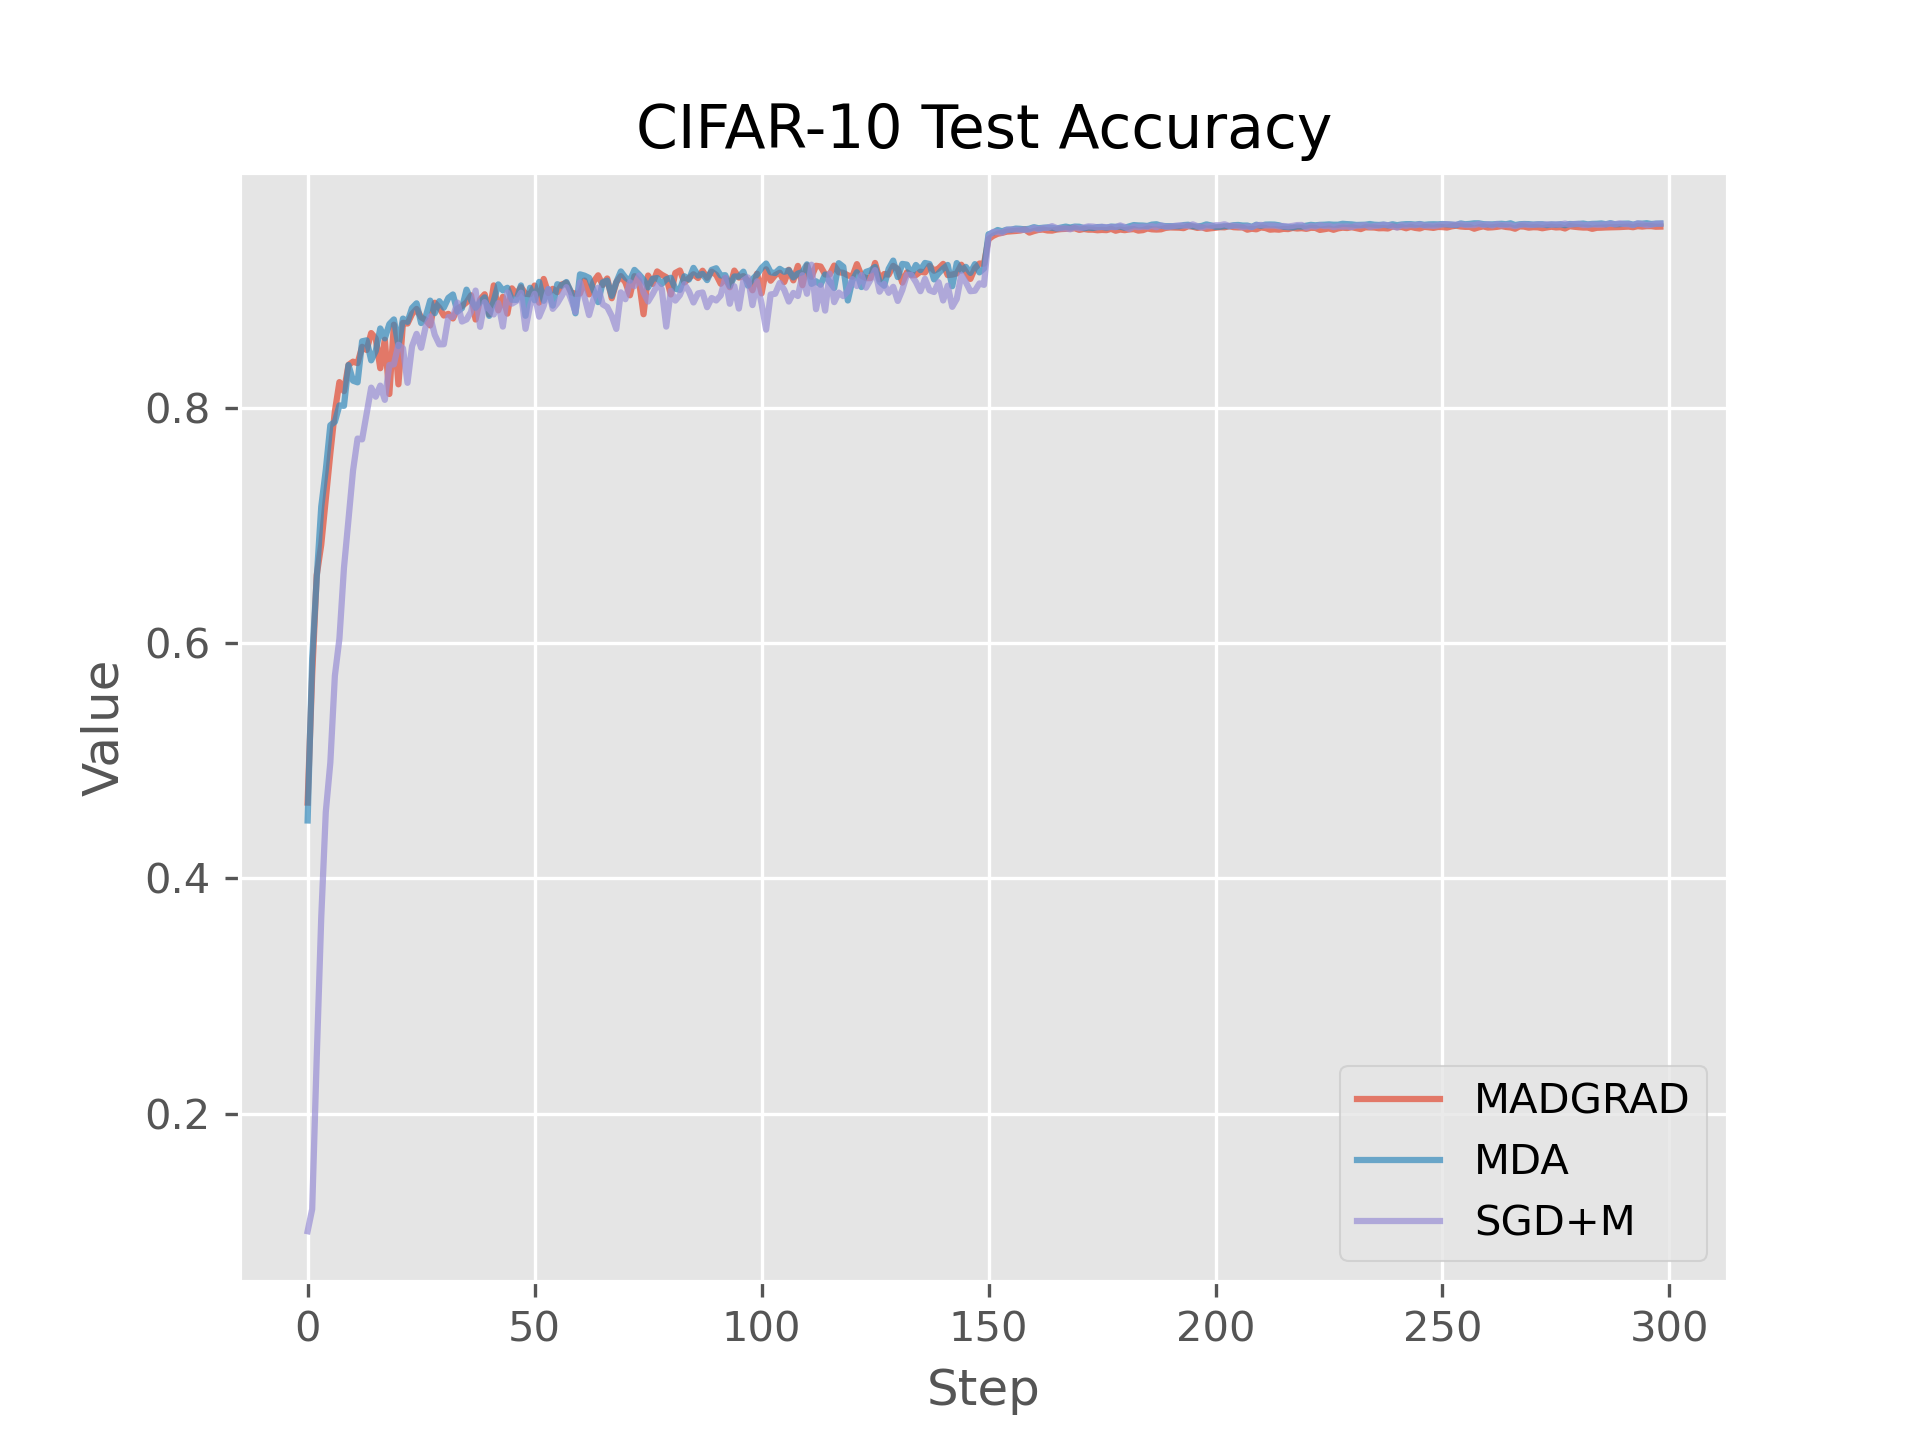
\includegraphics[width=\linewidth]{../ftrl_dl_data/CIFAR-10_test_acc.png}
    \caption{Test Accuracy of Optimizers on CIFAR-10}
    \label{fig:sub1}
  \end{subfigure}%
  \begin{subfigure}{.5\textwidth}
    \centering
    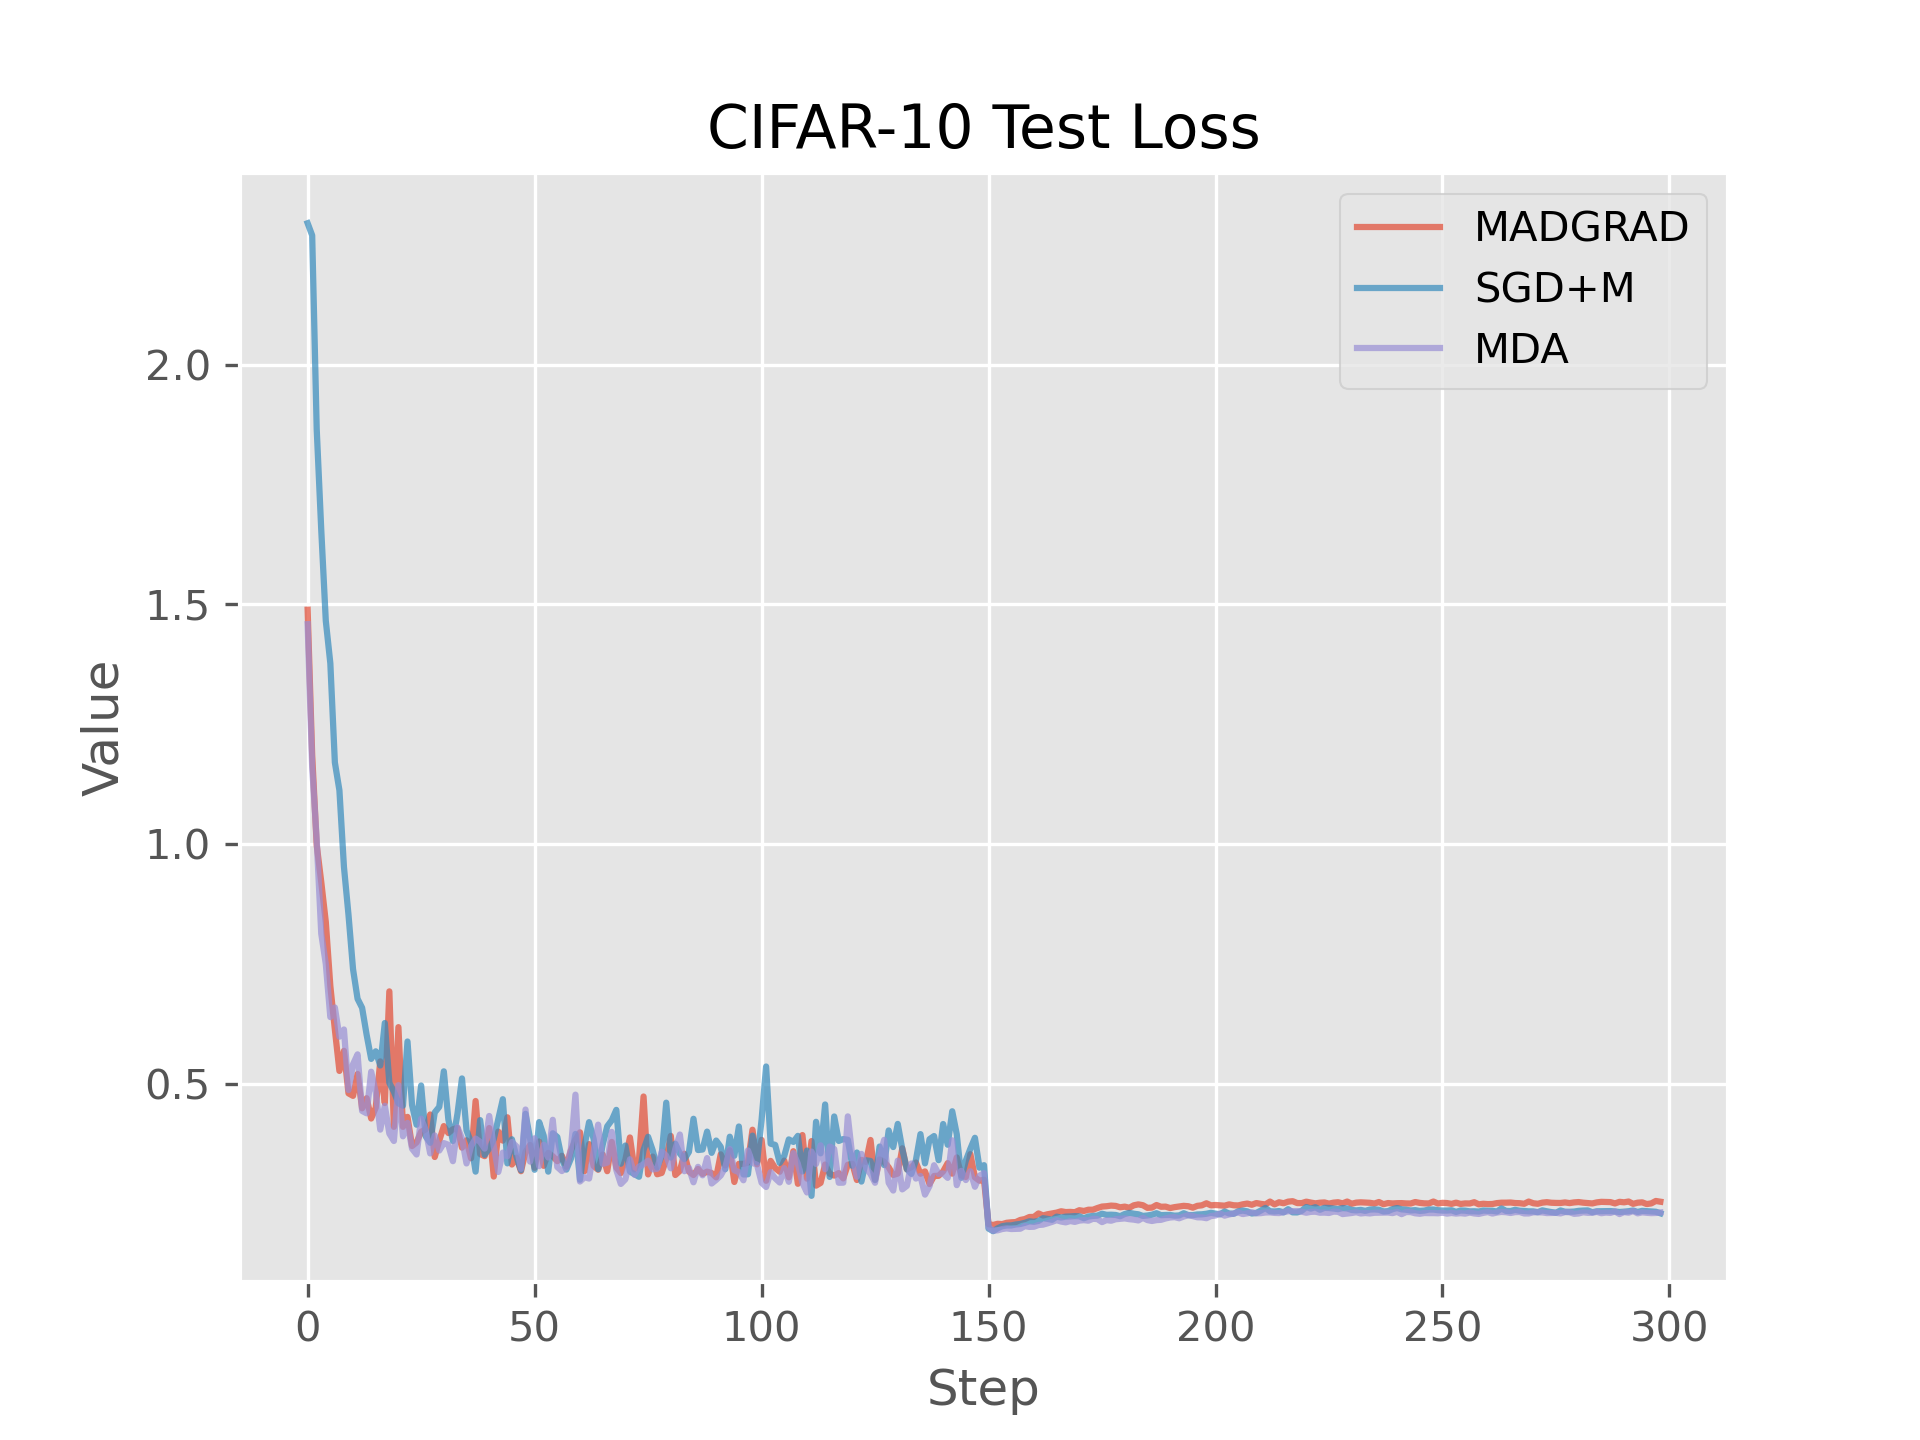
\includegraphics[width=\linewidth]{../ftrl_dl_data/CIFAR-10_test_loss.png}
    \caption{Test Loss of Optimizers on CIFAR-10}
    \label{fig:sub2}
  \end{subfigure}
  \caption{Comparison of optimizer performance on CIFAR-10 dataset}
  \label{fig:test}
\end{figure}

Our experiment setup and optimizer implementations for MDA and MADGRAD can be found at
\url{https://github.com/shashankmanjunath/ftrl_deep_learning}. We provide algorithm hyperparameters in~\ref{algoparams}.

Comparing algorithm performance shows that MDA and MADGRAD achieve performance on par with tuned SGD+M, and outperform
tuned Adam. However, MDA and MADGRAD also require significant parameter tuning in order to perform appropriately, and
therefore do not necessarily provide a significant advantage over SGD+M.

\section{Theory}\label{section:theory}

When proving the convergence bound for MADGRAD, the authors require an alternative definition of
MADGRAD than the one presented in the paper and implemented. In the original MADGRAD algorithm presented in the paper,
the $z_{k+1}$ is given by:

\[
  z_{k+1} = x_0 - \frac{1}{\sqrt[3]{v_{k+1}} + \epsilon} \circ s_{k+1}
\]

where $\circ$ indicates the Hadamard product. $\epsilon$ is included for numerical stability in the early iterations of
the algorithm, as the $v_{k+1}$ parameter can be 0. However, in the convergence proof, the $z_{k+1}$ parameter is given
by:

\[
  z_{k+1} = x_0 - \frac{1}{\sqrt[3]{\lambda_{k+1}G^2 + v_{k+1}}} \circ s_{k+1}
\]

Note the extra $\lambda_{k+1}G^2$ in the denominator, which is used to create the following upper bound leveraged in the
overall convergence proof proposed by the original authors:

\[
  \sum\limits_{t=0}^k \frac{\lambda_t^2 g_t^2}{\sqrt[3]{\lambda_t G^2 + \sum\limits_{i=0}^{t-1} \lambda_i g_i^2}} \leq
  \frac{3}{2} \lambda_k \left(\sum\limits_{i=1}^k \lambda_i g_i^2\right)^{\frac{2}{3}}
\]

This extra $\lambda_t G^2$ prevents the algorithm from being \emph{scale-free}, or an algorithm that is invariant to the
scaling of losses by a constant factor. Therefore, we aim to construct a convergence proof which maintains the
scale-free nature of the algorithm.

\subsection{Proof of Scale-Free Regret Bound for MADGRAD}

Consider the MADGRAD algorithm. This algorithm implements FTRL with the regularizer: 

\[
  \psi_t(\bx) = \frac{1}{2} \|\bx - \bx_0 \|_{A_t}
\]

where $A_t = \diag(\alpha_t)$, and $\alpha_t = \sqrt[3]{\sum_{i=1}^{t-1}\lambda_i g_i^2}$. Note that $\psi_t(\bx)$ is
strongly-convex with respect to the norm $\| \cdot \|_{A_t}$. Let us denote the Bregman divergence of a function $f$
over two vectors $\bx, \by \in \R^D$ by $B_f(\bx; \by)$ and let $f^*$ indicate the Fenchel conjugate of $f$. In
order to prove the scale-free bound, we make the reduction that $c_t = 1$ for all rounds. This effectively removes the
momentum operation, and leaves us with only FTRL iterates. Let us first make a useful proposition. Proving a scale-free
bound for the whole algorithm will require modification of Lemma~\ref{lemma:1} in order to handle the modified update.
Lemmas of this form are proved in (\cite{nesterov_quasi-monotone_2015}); however, we were not able to prove a specific
alternate lemma which would enable a robust convergence bound. Note that we make no assumption on the boundedness of our
convex set $K$ used as the feasible set for our algorithm. Additionally, we make no assumptions about the boundedness of
subgradients $g_i$. 

\begin{restatable}[Proposition 2 in~\cite{orabona_generalized_2014}: Properties of Fenchel Conjugates of
  Strongly Convex Functions]{proposition}{fenchelprop}\label{prop:1}
  Let $K \subseteq \R^D$ be a non-empty closed convex set. Let $\lambda \geq 0$, and let $f: K \rightarrow R$ be a lower
  semi-continuous function that is $\lambda$-strongly convex with respect to $\| \cdot \|$. The Fenchel conjugate of f
  satisfies:

  \begin{enumerate}
    \item $f^*$ is finite everywhere and differentiable
    \item $\nabla f^* (\ell) = \argmin_{w \in K}(f(w) - \langle \ell, w \rangle)$
    \item For any $\ell \in V^*$, $f^*(\ell) + f(\nabla f^*(\ell)) = \langle \ell, \nabla f^* (\ell) \rangle$
    \item $f^*$ is $\frac{1}{\lambda}$-strongly smooth, i.e.\ for any $x, y \in V^*$, $B_{f^*}(x, y) \leq
      \frac{1}{2\lambda}\|x - y \|_*$
    \item $f^*$ has $\frac{1}{\lambda}$-Lipschitz continuous gradients, i.e. $\| \nabla f^*(x) - \nabla f^*(y)\| \leq
      \frac{1}{\lambda}\|x - y\|_*$ for any $x, y \in V^*$
  \end{enumerate}
\end{restatable}

Let us now define some useful lemmas.

\begin{restatable}[Lemma 1 in~\cite{orabona_generalized_2014}]{lemma}{lemma1}\label{lemma:1}
  Let $\{\psi_t\}_{t=1}^\infty$ be a sequence of lower semi-continuos functions defined on a common convex domain $S
  \subseteq \R^n$ and such that each $\psi_t$ is $\mu_t$-strongly convex with respect to the norm $\|\cdot\|_t$. Let
  $\|\cdot\|_{t, *}$ be the dual norm of $\| \cdot \|_t$, for $t = 1, 2, \cdots, T$. Then, for any $\bu \in S$,

  \[
    \Regret _T (\bu) \leq \sum\limits_{t=1}^T \langle g_t, \bu - \bx_t \rangle \leq \psi_{T}(\bu) + \psi_{1}^* (0) +
    \sum\limits_{t=1}^T B_{\psi_{t}^*}(-\theta_t, -\theta_{t-1}) - \psi_{t}^* (-\theta_t) +
    \psi_{t+1}^*(-\theta_t)
  \]
\end{restatable}

\proof~Given in (\cite{orabona_generalized_2014})
\qed

\begin{restatable}{lemma}{firstbound}\label{lemma:2}
  Let $a_1, a_2, \cdots, a_t$ be non-negative real numbers. If $a_1 > 0$, then
  \[
    \sum\limits_{t=1}^T \frac{a_t}{\sqrt[3]{\sum\limits_{s=1}^t a_s}} \leq \frac{3}{2}\left(\sum\limits_{t=1}^T
    a_t\right)^\frac{2}{3}
  \]
\end{restatable}

\proof~Given in~\ref{lemmaproof:2}

\begin{restatable}{lemma}{secondbound}\label{lemma:3}
  Let $C, a_1, a_2, \cdots, a_T \geq 0$, and $\alpha \geq 1, \alpha \neq \min\limits_{t=1,2,\cdots,T}a_{t}^\frac{4}{3}$.
  Then,

  \[
    \sum\limits_{t=1}^T \min \left\{ \frac{a_{t}^2}{\sqrt[3]{\sum\limits_{s=1}^{t-1} a_{s}^2}}, C a_t\right\} \leq
    \frac{C \alpha}{\alpha - \min\limits_{t=1,2,\cdots,T}a_{t}^\frac{4}{3}} \max\limits_{t=1,2,\cdots,T} a_t
    + 2\sqrt[3]{1 + \alpha^2} \sqrt{\sum\limits_{s=1}^T a_{s}^3}
  \]
\end{restatable}

\proof~Given in~\ref{lemmaproof:3}

Let us now state the overall convergence bound for our version of MADGRAD. Our proof of this technique broadly follows
the technique set forth for Scale-Free Online Linear Optimization FTRL given in (\cite{orabona_scale-free_2015}) applied
in a per-coordinate manner. We additionally only handle the constant learning rate case, which ensures that $\lambda_t
\leq \lambda_{t+1}$

\begin{restatable}{theorem}{regretbound}\label{theorem:1}
  Suppose $K \subseteq \R^D$ is a non-empty closed convex subset. Suppose that a regularizer $\psi_t: K \rightarrow \R$
  is a non-negative lower semi-continuous function that is strongly convex with respect to a norm $\| \cdot
  \|_{A_t}$. The regret of non-momentumized MADGRAD satisfies:

  \begin{align*}
    \Regret_T(\bu) \leq \sum\limits_{d=1}^D \frac{(\bu_d - x_{0,d})^2}{2\sqrt[3]{\sum\limits_{i=1}^{T} \lambda_i
        g_{i,d}^2}} + \frac{3}{2}\left(\sum\limits_{i=1}^T \lambda_i g_{i,d}^2\right)^\frac{2}{3} +& 2
        \sqrt{T-1}\left(\sum_{i=1}^{T-1} \lambda_i g_{i,d}^2\right)^\frac{2}{3}(1 + \min_{t \leq
        T}(\sqrt{\lambda_t}|g_{t,d}|)^\frac{4}{3}) \max_{t \leq T} \sqrt{\lambda_t}|g_{td}| \\ &+ 2\sqrt[3]{1 + (1 +
        \min_{t \leq T}(\sqrt{\lambda_t}|g_{t,d}|)^\frac{4}{3})^2}\sqrt{\sum\limits_{t-1}^T \lambda_t^\frac{3}{2}
      |g_{t,d}|^3}
  \end{align*}
\end{restatable}

\proof Note that $\psi_t (x) = \frac{1}{2} \| \bx - \bx_0\|_{A_t}^2$, where $A_t = \diag(\alpha_t)$. For this
regularizer, $\alpha_t = \sqrt[3]{\sum\limits_{i=1}^{t-1} \lambda_i g_{i}^2} \in \R^D$. Let $L_t = \sum\limits_{i=1}^t
\lambda_i g_i$. Let us perform this analysis per-coordinate.

\[
  \psi_{t,d}(\bx) = \frac{1}{2} (\bx_d - \bx_{0,d})\sqrt[3]{\sum\limits_{i=1}^{t-1} \lambda_i g_{id}^2}(\bx_d -
  \bx_{0,d}) = \frac{1}{2}\sqrt[3]{\sum\limits_{i=1}^{t-1} \lambda_i g_{id}^2}(\bx_d - \bx_{0,d})^2.
\]

Let $\eta_{t,d} = \frac{1}{\sqrt[3]{\sum\limits_{i=1}^{t-1} \lambda_i g_{id}^2}}$. Therefore, we have:

\begin{align*}
  \psi_{t,d} (\bx) &= \frac{1}{\eta_{t,d}} \psi_d(\bx) \\
  \psi_d(\bx) &= \frac{1}{2} (\bx_d - \bx_{0,d})^2
\end{align*}

Since $A_t$ is a diagonal matrix, $\psi_t(\bx)$ is $\min_{d \leq D} \sqrt[3]{\sum\limits_{i=1}^{t-1} \lambda_i
g_{i,d}^2}$-strongly convex. We can tighten this bound by analyzing $\psi_{t,d}(\bx)$ and establishing a per-coordinate
strong convexity bound. Recall that, since $\psi_d(\bx): \R \rightarrow \R$, we can find the strong convexity constant
by finding the lower bound of the second derivative of $\psi_d(\bx)$.

\begin{align*}
  \frac{d \psi_d(\bx)}{d \bx_d} &= \bx_d - \bx_{0,d} \\
  \frac{d^2 \psi_d(\bx)}{d \bx_d^2} &= 1
\end{align*}

Therefore, $\psi_d(\bx)$ is 1-strongly convex with respect to $| \cdot |$, as we are dealing with real numbers in the
per-coordinate case. By Lemma 1, we have:

\[
  \Regret_T(\bu) \leq \psi_{T+1}(\bu) + \psi_{1}^* (\textbf{0}) + \sum\limits_{t=1}^T B_{\psi_{t}^*}(-L_t,
  -L{t-1}) - \psi_{t}^* (-L_t) + \psi_{t-1}^*(-L_t)
\]

Writing this in a per-coordinate manner,

\begin{align*}
  \Regret_T(\bu) 
  &\leq \sum\limits_{d=1}^D \psi_{T+1,d}(\bu) + \psi_{1,d}^* (\textbf{0}) + \sum\limits_{t=1}^T
  B_{\psi_{t,d}^*}(-L_t, -L{t-1}) - \psi_{t,d}^* (-L_t) + \psi_{t-1,d}^*(-L_t) \\
  &\leq \sum\limits_{d=1}^D \frac{1}{\eta_{T+1}}\psi_{d}(\bu) + \frac{1}{\eta_1}\psi_{d}^* (\textbf{0}) + \sum\limits_{t=1}^T
  B_{\psi_{t,d}^*}(-L_t, -L{t-1}) - \psi_{t,d}^* (-L_t) + \psi_{t-1,d}^*(-L_t)
\end{align*}

Let us proceed by bounding $B_{\psi_{t,d}^*}(-L_t, -L{t-1}) - \psi_{t,d}^* (-L_t) + \psi_{t-1,d}^*(-L_t)$ in
two ways.

\begin{enumerate}
  \item By Proposition \ref{prop:1} item 4, we know that $B_{\psi_{t,d}^*}(-L_t, -L_{t-1}) \leq \frac{\eta_t \lambda_t
    g_{t,d}^2}{2 \mu_{t,d}} = \frac{\eta_t \lambda_t g_{t,d}^2}{2}$. Therefore, by Lemma \ref{lemma:1}, we know that:

    \[
      B_{\psi_{t,d}^*}(-L_t, -L_{t-1}) - \psi_{t,d}^*(-L_t) + \psi_{t+1,d}^*(-L_t) \leq B_{\psi_{t,d}^*}(-L_t,
      -L_{t-1}) \leq \frac{\eta_t \lambda_t g_{t,d}^2}{2}
    \]

    since $\psi_{t,d}^* \geq \psi_{t+1,d}^*$.
  \item Similarly,

    \begin{align*}
      B_{\psi_{t,d}^*}(-L_t, -L_{t-1}) 
      &- \psi_{t,d}^*(-L_t) + \psi_{t+1,d}^*(-L_t) = B_{\psi_{t+1,d}^*}(-L_t, -L_{t-1}) + \psi_{t+1,d}^*(-L_{t-1}) \\
      & - \psi_{t,d}^*(-L_{t-1}) + \langle \nabla \psi_{t,d}^*(-L_{t-1}) - \nabla \psi_{t+1,d}^*(-L_{t-1},
      g_{t,d}))\rangle \\
      &\leq \frac{1}{2} \eta_{t+1,d}\lambda_t g_{t,d}^2 + | \nabla \psi_{t,d}^*(-L_{t-1}) - \nabla
      \psi_{t+1,d}^*(-L_{t-1})| |g_{t,d}| \\
      &\leq \frac{1}{2} \eta_{t+1,d}\lambda_t g_{t,d}^2 + | \nabla \psi_{d}^*(-\eta_{t,d} L_{t-1}) - \nabla
      \psi_{d}^*(-\eta_{t+1}L_{t-1})| |g_{t,d}| \\
      &\leq \frac{1}{2} \eta_{t+1,d}\lambda_t g_{t,d}^2 + |L_{t-1}|(\eta_{t,d} - \eta_{t+1,d})|g_{t,d}|
    \end{align*}

    Recall that $\eta_{t,d} = \frac{1}{\sqrt[3]{\sum\limits_{i=1}^{t-1} \lambda_i g_{id}^2}}$. Therefore,

    \begin{align*}
      |L_{t-1}|(\eta_{t,d} - \eta_{t+1,d}) 
      &\leq |L_{t-1}|\eta_{t,d} = \frac{\sum_{i=1}^{t-1} \lambda_i g_{i,d}}{\sqrt[3]{\sum_{i=1}^{t-1}\lambda_i
      g_{i,d}^2}} \\
      &\leq \frac{\sqrt{(\sum_{i=1}^{t-1} \sqrt{\lambda_i} g_{i,d}
      \sqrt{\lambda_i})^2}}{\sqrt[3]{\sum_{i=1}^{t-1} \lambda_i g_{i,d}^2}} \\
      &\leq \frac{\sqrt{(\sum_{i=1}^{t-1} \lambda_i)(\sum_{i=1}^{t-1}\lambda_i g_{i,d}^2)}}{\sqrt[3]{\sum_{i=1}^{t-1} \lambda_i g_{i,d}^2}}
    \end{align*}

    By Callebaut's inequality. Therefore, we have:

    \[
      |L_{t-1}|(\eta_{t,d} - \eta_{t+1,d}) \leq \left(\sqrt{\sum_{i=1}^{t-1} \lambda_i}\right)\left(\sum_{i=1}^{t-1}\lambda_i
      g_{i,d}^2\right)^\frac{2}{3}
    \]
\end{enumerate}

Combining these two bounds, we have:

\[
  B_{\psi_{t,d}^*}(-L_t, -L_{t-1}) - \psi_{t,d}^*(-L_t) + \psi_{t+1,d}^*(-L_t) \leq \frac{\eta_t \lambda_t g_{t,d}^2}{2}
  + \left(\sqrt{\sum_{i=1}^{t-1} \lambda_i}\right)\left(\sum_{i=1}^{t-1}\lambda_i g_{i,d}^2\right)^\frac{2}{3}
\]

Note that 
\[
  \sqrt{\sum\limits_{i=1}^{t-1}\lambda_i} \leq \sqrt{(t-1) \lambda_t} = \sqrt{t-1}\sqrt{\lambda_t}
\]

Let $H = \left(\sum\limits_{i=1}^{t-1} \lambda_i g_{i,d}^2\right)^\frac{2}{3} \sqrt{t-1}$. Therefore, we have:

\[
  B_{\psi_{t,d}^*}(-L_{t}, -L_{t-1}) - \psi_{t,d}^*(-L_t) + \psi_{t+1,d}^*(-L_t) \leq \frac{\eta_{t+1,d} \lambda_t
  g_{t,d}^2}{2} + H \sqrt{\lambda_t}|g_{t,d}|
\]

Therefore, we have an overall regret bound of

\begin{align}
  \Regret_T(\bu) 
  &\leq \sum\limits_{d=1}^D \frac{1}{\eta_{T+1}}\psi_{d}(\bu) + \frac{1}{\eta_1}\psi_{d}^*(0)+\sum\limits_{t=1}^T \min
  \left\{\frac{\eta_t \lambda_t g_{t,d}^2}{2}, \frac{\eta_{t+1,d} \lambda_t g_{t,d}^2}{2} + H
  \sqrt{\lambda_t}|g_{t,d}|\right\} \nonumber \\
  \therefore \Regret_T(\bu) 
  &\leq \frac{1}{\eta_{T+1}}\psi_{d}(\bu) + \frac{1}{\eta_1}\psi_{d}^*(0)+\frac{1}{2}\sum\limits_{t=1}^T \eta_{t+1}
  \lambda_t g_{t,d}^2 + \frac{1}{2}\sum\limits_{t=1}^T \min \left\{\frac{\eta_t \lambda_t g_{t,d}^2}{2},  2H
  \sqrt{\lambda_t}|g_{t,d}|\right\} \label{eq:1}
\end{align}

Let us bound this regret in three groups.

\begin{enumerate}
\item $\frac{1}{2}\sum\limits_{t=1}^T \min \left\{\frac{\eta_t \lambda_t g_{t,d}^2}{2}, 2H\sqrt{\lambda_t}|g_{t,d}|\right\}$

  We bound this using Lemma \ref{lemma:3}. Let $B = \min_{t\leq T}a_{t}^\frac{4}{3}$ setting $\alpha = 1+B$.
  \[
    \frac{1}{2}\sum\limits_{t=1}^T \min \left\{\frac{\eta_t \lambda_t g_{t,d}^2}{2}, 2H\sqrt{\lambda_t}|g_{t,d}|\right\}
    \leq 2H(1+B)\max_{t\leq T}\sqrt{\lambda_t}|g_{t,d}| +
    2\sqrt[3]{1 + (1+B)^2}\sqrt{\sum\limits_{t=1}^T \lambda_{t}^\frac{3}{2} g_{t,d}^3}
  \]
\item $\sum\limits_{t=1}^T \frac{\lambda_t g_{t,d}^2}{\sqrt[3]{\sum\limits_{i=1}^t}\lambda_i g_{i,d}^2}$. We bound this
  by Lemma \ref{lemma:2}.

  \[
    \sum\limits_{t=1}^T \frac{\lambda_t g_{t,d}^2}{\sqrt[3]{\sum\limits_{i=1}^t\lambda_i g_{i,d}^2}} \leq \frac{3}{2}
    \left(\sum\limits_{t=1}^T \lambda_t g_{t,d}^2\right)^\frac{2}{3}
  \]
\item $\frac{1}{\eta_{T+1}}\psi_{d}(\bu) + \frac{1}{\eta_1}\psi_{d}^*(0)$.

  Note that $\psi_d(\bu) = \frac{1}{2}(\bu_d - x_{0,d})$. Therefore,

  \[
    \frac{1}{\eta_{T+1,d}}\psi_d(\bu) = \frac{(\bu_d - x_{0,d})^2}{2 \sqrt[3]{\sum\limits_{t=1}^T \lambda_i g_{i,d}^2}}
  \]

  Now let us analyze $\psi_d^*(0)$. By Proposition \ref{prop:1} item 2,

  \begin{align*}
    \psi_d^*(0) = \sup\limits_{x \in K}(\langle x , 0 \rangle - \psi_d(x)) = \sup_{x \in K}(-\frac{1}{2}(\bx_d -
    x_{0,d})) \leq 0
  \end{align*}

  Therefore, $\frac{1}{\eta_{T+1}}\psi_{d}(\bu) + \frac{1}{\eta_1}\psi_{d}^*(0) \leq \frac{1}{\eta_{T+1}}\psi_{d}(\bu)$
\end{enumerate}

Substituting these three upper bounds back into (\ref{eq:1}) gives the desired bound. \\
\qed

\section{Conclusion}

In this work, we have tested implementations of the MADGRAD and MDA algorithms, and proved a convergence bound for
non-momentumized MADGRAD. Future work includes proving a convergence bound for momentumized MADGRAD.

\newpage

\bibliographystyle{plainnat}
\bibliography{project_report}

\newpage

\appendix
\section{Appendix}
\subsection{Algorithm Parameters}\label{algoparams}

We set our parameters as described in~\cite{defazio_adaptivity_nodate}, following standard practice. Our data
augmentation pipeline includes random horizontal flipping, random cropping to 32x32, then normalization by centering
around (0.5, 0.5, 0.5).

\begin{center}
  \begin{tabular}{ | l | l | }
  \hline
  \textbf{Hyperparameter} & \textbf{Value} \\
  \hline
  Architecture & PreAct ResNet152 \\
  \hline
  Epochs & 300 \\
  \hline
  GPUs & 1x A100 \\
  \hline
  Batch Size per GPU & 128 \\
  \hline
  Learning Rate Schedule & 150-225 tenthing \\
  \hline
\end{tabular}
\end{center}

\begin{center}
  \begin{tabular}{ | l | l | l |}
    \hline
    Method & Learning Rate & Decay \\
    \hline
    MADGRAD & 2.5e-4 & 0.0001 \\
    \hline
    MDA & 2.5e-4 & 0.0001 \\
    \hline
    Adam & 2.5e-4 & 0.0001 \\
    \hline
    SGD+M & 0.1 & 0.0001 \\
    \hline
  \end{tabular}
\end{center}

\subsection{Proof of Lemma 2}\label{lemmaproof:2}

\firstbound*

\proof Note that if $0 \leq x \leq 1$, 

\[
  \frac{2}{3} x \leq 1 - (1 - x)^\frac{2}{3}
\]

Let $L_t = \sum\limits_{i=1}^t \ell_i$, and let $x = \frac{\ell_t}{L_t}$. Let $\ell_0 = 0$.

\begin{align*}
  \frac{2}{3} \frac{\ell_t}{L_t}
  &\leq 1 - (1 - \frac{\ell_t}{L_t})^\frac{2}{3} = 1 - (\frac{L_{t-1}}{L_t})^\frac{2}{3} \\
  \frac{2}{3} \frac{\ell_t}{L_t} L_{t}^\frac{2}{3} &\leq L_{t}^\frac{2}{3} - L_{t-1}^\frac{2}{3} \\
  \frac{2}{3} \frac{\ell_t}{\sqrt[3]{L_t}} &\leq L_{t}^\frac{2}{3} - L_{t-1}^\frac{2}{3} \\
  \therefore \frac{2}{3} \sum\limits_{t=1}^T \frac{\ell_t}{\sqrt[3]{L_t}} &\leq \sum\limits_{t=1}^T L_{t}^\frac{2}{3} -
  L_{t-1}^\frac{2}{3} \\
  \sum\limits_{t=1}^T \frac{\ell_t}{\sqrt[3]{L_t}} &\leq \frac{3}{2} L_{T}^\frac{3}{2} \\
  \sum\limits_{t=1}^T \frac{\ell_t}{\sqrt[3]{L_t}} &\leq \frac{3}{2} \left(\sum\limits_{t=1}^T \ell_t \right)^\frac{2}{3}
\end{align*}

Letting $\ell_i = a_i \forall i$ yields the lemma.

\qed

\subsection{Proof of Lemma 3}\label{lemmaproof:3}

\secondbound*

\proof We will prove this bound by proving each individual case in the minimum, then summing them.

\emph{Case 1}. Consider $a_t \leq \alpha^3 \left(\sum\limits_{s=1}^{t-1} a_s^2\right)^\frac{2}{3}$.

\begin{align*}
  \min \left\{ \frac{a_{t}^2}{\sqrt[3]{\sum\limits_{s=1}^{t-1} a_{s}^2}}, C a_t \right\} 
  &\leq \frac{\alpha_{t}^2}{\sqrt[3]{\sum\limits_{s=1}^{t-1}a_{s}^2}} =
  \frac{a_{t}^2}{\sqrt[3]{\frac{1}{1+\alpha^2}\left(\alpha^2 \sum\limits_{s=1}^{t-1} a_{s}^2 +
  \sum\limits_{s=1}^{t-1} a_{s}^2 \right)}} \\
  &\leq \frac{a_{t}^2 \sqrt[3]{1 + \alpha^2}}{\sqrt[3]{a_{t}^2 + \sum\limits_{s=1}^{t-1} a_{s}^2}} = \frac{a_{t}^2
  \sqrt[3]{1 + \alpha^2}}{\sqrt[3]{\sum\limits_{s=1}^t a_{s}^2}}
\end{align*}

Note that $\frac{x^2}{\sqrt[3]{x^2 + y^2}} \leq 2(\sqrt{x^3 + y^3} - \sqrt{y^3})$. Using this inequality,

\[
  \sqrt[3]{1 + \alpha^2} \frac{a_{t}^2}{\sqrt[3]{\sum\limits_{s=1}^t a_{s}^2}} \leq 2 \sqrt[3]{1 +
  \alpha^2}\left(\sqrt{\sum\limits_{s=1}^t a_{s}^3} - \sqrt{\sum\limits_{s=1}^{t-1} a_{s}^3}\right)
\]

\emph{Case 2} Consider $a_{t}^2 \geq \alpha^3 \left(\sum\limits_{s=1}^{t-1} a_{s}^2\right)^\frac{2}{3}$. Note that this
implies that $a_t \geq \alpha^\frac{3}{2} \sqrt[3]{\sum\limits_{s=1}^{t-1} a_{s}^2}$. Additionally, let 
$A = \left( \sum\limits_{s=1}^{t-1} a_{s}^2 \right)^\frac{2}{3}$.


\begin{align*}
  \min \left\{ \frac{a_{t}^2}{\sqrt[3]{\sum\limits_{s=1}^{t-1} a_{s}^2}}, C a_t \right\}
  &\leq C a_t = C a_t \left(\frac{\alpha - A}{\alpha -A}\right) \\
  &\leq \frac{C}{\alpha - A}\left(\alpha a_t - A a_t\right) = \frac{C \alpha}{\alpha - A}\left(a_t - \alpha^\frac{1}{2}
    A \sqrt[3]{\sum\limits_{s=1}^{t-1} a_{s}^2}\right) \\
  &\leq \frac{C \alpha}{\alpha - A}\left(a_t - \left( \sum\limits_{s=1}^{t-1} a_{s}^2 \right)^\frac{2}{3}
  \left(\sum\limits_{s=1}^{t-1} a_{s}^2\right)^\frac{1}{3}\right) \\
  &\leq \frac{C \alpha}{\alpha - A}\left(a_t - \sqrt{\sum\limits_{s=1}^{t-1} a_{s}^2}\right)
\end{align*}

Let $M_t = \max \{a_t, \cdots, a_t\}$. Note that in this case, $a_t = M_t$, and $\sqrt{\sum\limits_{s=1}^{t-1} a_{s}^2}
\geq M_{t-1}$. Therefore,

\[
  \min \left\{ \frac{a_{t}^2}{\sqrt[3]{\sum\limits_{s=1}^{t-1} a_{s}^2}}, C a_t \right\} \leq 
  \frac{C \alpha}{\alpha - A}\left(M_t - M_{t-1}\right)
\]

Further note that since $a_t \geq 0 \forall t$, $A = (\sum\limits_{s=1}^T a_{s}^2)^\frac{2}{3} \geq
\min_{t=1,\cdots,T}a_{t}^\frac{4}{3}$. Let $B = \min_{t=1,\cdots,T}a_{t}^\frac{4}{3}$, Therefore,

\[
  \min \left\{ \frac{a_{t}^2}{\sqrt[3]{\sum\limits_{s=1}^{t-1} a_{s}^2}}, C a_t \right\} \leq 
  \frac{C \alpha}{\alpha - B}\left(M_t - M_{t-1}\right)
\]

Therefore, combining the two cases, we have:

\[
  \min \left\{ \frac{a_{t}^2}{\sqrt[3]{\sum\limits_{s=1}^{t-1} a_{s}^2}}, C a_t \right\} \leq \frac{C \alpha}{\alpha -
  B}\left(M_t - M_{t-1}\right) + 2 \sqrt[3]{1 + \alpha^2}\left(\sqrt{\sum\limits_{s=1}^t a_{s}^3} -
  \sqrt{\sum\limits_{s=1}^{t-1} a_{s}^3}\right)
\]

Therefore, summing from $t=1$ to $T$,

\[
  \sum\limits_{t=1}^T\min \left\{ \frac{a_{t}^2}{\sqrt[3]{\sum\limits_{s=1}^{t-1} a_{s}^2}}, C a_t \right\} \leq \frac{C
  \alpha}{\alpha - B}\left(\max\limits_{t=1, \cdots, T} a_t\right) + 2 \sqrt[3]{1 +
  \alpha^2}\left(\sqrt{\sum\limits_{t=1}^T a_{t}^3}\right)
\]

\qed

\end{document}
